\documentclass[arhiv]{izpit}
\usepackage{fouriernc}
\usetikzlibrary{calc}
\renewcommand{\ttdefault}{txtt}

\begin{document}

\izpit{Programiranje I: 2.~izpit}{7.~maj 2013}{
  Čas reševanja je 120 minut.
  Veliko uspeha!
}

%%%%%%%%%%%%%%%%%%%%%%%%%%%%%%%%%%%%%%%%%%%%%%%%%%%%%%%%%%%%%%%%%%%%%%
\naloga[25 točk]

V \emph{Mathematici} lahko sprehod v ravnini predstavimo s seznamom korakov
$\mathtt{\{\{e_1, d_1\}, \dots, \{e_n, d_n\}\}}$,
  kjer so $\mathtt{e_i}$ enotski vektorji, ki predstavljajo smeri korakov,
  $\mathtt{d_i}$ pa pozitivna realna števila, ki predstavljajo njihove dolžine.

\podnaloga
Sestavite funkcijo \verb|naloga1a[sez_]|,
  ki vrne točke, ki jih obišče sprehod,
  podan s seznamom korakov \verb|sez| v gornji obliki.

{\small\begin{verbatim}
   In[1]:= naloga1a[{{{0, 1}, 2}, {{1, 0}, 1}, {{-1, 0}, 4}}]
   Out[1]= {{0, 0}, {0, 2}, {1, 2}, {-3, 2}}
   In[2]:= naloga1a[{{{0, 1}, 2}, {{1, 0}, 1}, {{-1, 0}, 4}, {{3/5, 4/5}, 5}}]
   Out[2]= {{0, 0}, {0, 2}, {1, 2}, {-3, 2}, {0, 6}}\end{verbatim}}

\podnaloga
Sestavite funkcijo \verb|naloga1b[sez_]|,
  ki iz seznama obiskanih točk \verb|sez| izračuna
  seznam korakov v gornji obliki.

{\small\begin{verbatim}
   In[3]:= naloga1b[{{0, 0}, {0, 2}, {1, 2}, {-3, 2}}]
   Out[3]= {{{0, 1}, 2}, {{1, 0}, 1}, {{-1, 0}, 4}}
   In[4]:= naloga1b[{{0, 0}, {0, 2}, {1, 2}, {-3, 2}, {0, 6}}]
   Out[4]= {{{0, 1}, 2}, {{1, 0}, 1}, {{-1, 0}, 4}, {{3/5, 4/5}, 5}}\end{verbatim}}

%%%%%%%%%%%%%%%%%%%%%%%%%%%%%%%%%%%%%%%%%%%%%%%%%%%%%%%%%%%%%%%%%%%%%%
\naloga[25 točk]

Vsako dvojiško drevo lahko razdelimo na plasti tako,
  da so v prvi plasti vsi listi drevesa,
  v drugi plasti vsa vozlišča, ki imajo otroke v prvi plasti,
  in tako naprej.
Primer razdelitve drevesa na plasti:
\[
  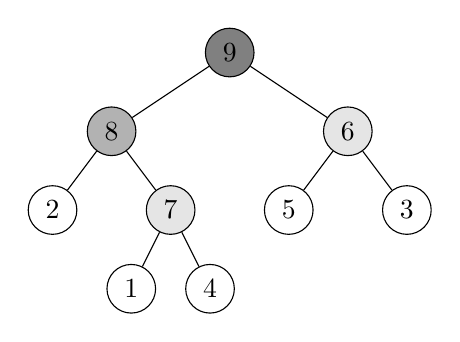
\begin{tikzpicture}[level distance=1cm,
    level 1/.style={sibling distance=3cm},
    level 2/.style={sibling distance=1.5cm},
    level 3/.style={sibling distance=1cm}
    ]
    \node[circle, draw, fill=black!50] (d) {9}
      child {node[circle, draw, fill=black!30] {8}
        child {node[circle, draw] {2}}
        child {node[circle, draw, fill=black!10] {7}
          child {node[circle, draw] {1}}
          child {node[circle, draw] {4}}
        }
      }
      child {node[circle, draw, fill=black!10] {6}
        child {node[circle, draw] {5}}
        child {node[circle, draw] {3}}
      };
  \end{tikzpicture}
\]
%
Razredu \verb|Drevo| dodajte metodo \verb|naloga2(self, n)|,
  ki vrne množico vrednosti vseh vozlišč v plasti \verb|n|.
Metoda naj drevesa ne spreminja.

Pri zgornjem drevesu \verb|d| tako torej velja:
{\small\begin{verbatim}
   >>> d.naloga2(1)
   {1, 2, 3, 4, 5}
   >>> d.naloga2(2)
   {6, 7}
   >>> d.naloga2(3)
   {8}\end{verbatim}}

%%%%%%%%%%%%%%%%%%%%%%%%%%%%%%%%%%%%%%%%%%%%%%%%%%%%%%%%%%%%%%%%%%%%%%
\naloga[25 točk]
V \emph{Mathematici} sestavite funkcijo \verb|naloga3[n_]|,
  ki izriše sledeče fraktale:

\begin{center}
  
\includegraphics[width=\textwidth]{drevesa.pdf} \\
  \verb|naloga3[1]|\qquad
  \verb|naloga3[2]|\qquad
  \verb|naloga3[3]|\qquad
  \verb|naloga3[4]|\qquad
  \verb|naloga3[5]|
\end{center}

%%%%%%%%%%%%%%%%%%%%%%%%%%%%%%%%%%%%%%%%%%%%%%%%%%%%%%%%%%%%%%%%%%%%%%
\naloga[25 točk]

Sestavite funkcijo \verb|naloga4(t)|, ki za tabelo \verb|t| oblike
\[
  [a_k, a_{k + 1}, \dots, a_n, a_1, a_2, \dots, a_{k - 1}],
\]
kjer velja
\[
  a_1 < a_2 < \cdots < a_n,
\]
v času $O(\log n)$ poišče število $k$.

% Lomljeno črto lahko predstavimo s seznamom parov koordinat njenih točk.
% V \emph{Pythonu} sestavite funkcijo \verb|naloga4(sez)|, ki vrne \verb|True|,
%   kadar lomljena črta, ki poteka skozi točke iz seznama \verb|sez|, seka samo sebe,
%   in \verb|False|, kadar ne.
% Časovna zahtevnost funkcije naj bo $O(n \log n)$,
%   kjer je $n$ velikost seznama \verb|sez|.

% \[
%   \begin{tikzpicture}[scale=0.8]
%     \draw (-4.2,0) -- (4.2,0);
%     \draw (0,-4.2) -- (0,4.2);
%     \foreach \x in {-4,-3,...,4} {
%       \draw (\x,2pt) -- (\x,-2pt);
%       \draw (2pt,\x) -- (-2pt,\x);
%     }
%         \draw[thick] (-2, -2) -- (-3, -1) -- (-3, 2) -- (-2, 1) -- (1, 1) -- (3, 2) -- (3, -1);
%     \draw[thick] (-2, -1) -- (2, -3) -- (2, 1) -- (-1, -3);
%   \end{tikzpicture}
% \]


%   {\small\begin{verbatim}
%      >>> naloga4([(-2, -2), (-3, -1), (-3, 2), (-2, 1), (1, 1), (3, 2), (3, -1)])
%      False
%      >>> naloga4([(-2, -1), (2, -3), (2, 1), (-1, -3)])
%      True\end{verbatim}}


\end{document}

